% $Header: /cvsroot/latex-beamer/latex-beamer/solutions/generic-talks/generic-ornate-15min-45min.en.tex,v 1.5 2007/01/28 20:48:23 tantau Exp $

\documentclass{beamer}

\mode<presentation>
{
  \usetheme{Madrid}

  \setbeamercovered{invisible}
}

\usepackage[english]{babel}

\usepackage[latin1]{inputenc}

\usepackage{times}
\usepackage[T1]{fontenc}
\usepackage{graphicx}
\usepackage{subfigure}

% \renewcommand{\thesubfigure}{\thefigure.\arabic{subfigure}}
\renewcommand{\thesubfigure}{}

\title[Augmented Reality on FPGA]{Augmented Reality on FPGA}
\subtitle{Realtime Object Recognition and Image Processing}
\author[Logan Williams \and Jos\'{e} Cruz Serrall\'{e}s]{Logan Williams \and Jos\'{e} E. Cruz Serrall\'{e}s}

\date{15 November 2011}
\institute[6.111]{6.111 Fall 2011}


%\AtBeginSubsection[]
%{
%	\begin{frame}<beamer>{Outline}
%		\tableofcontents[currentsection,currentsubsection]
%	\end{frame}
%}

%\beamerdefaultoverlayspecification{<+->}

\begin{document}


\begin{frame}
	\titlepage
\end{frame}

\section{Introduction}
% Logan
\begin{frame}
	\frametitle{Introduction}
	\begin{itemize}
		\item Overlay a digital image on a physical object in realtime.
		\item In this case, we want to identify a picture frame in captured video, and output video with another image distorted to fit on top of the picture frame.
	\end{itemize}
\end{frame}

% Logan
\begin{frame}
% example output image
	\frametitle{Example Image}
	\begin{figure}
		\centering
		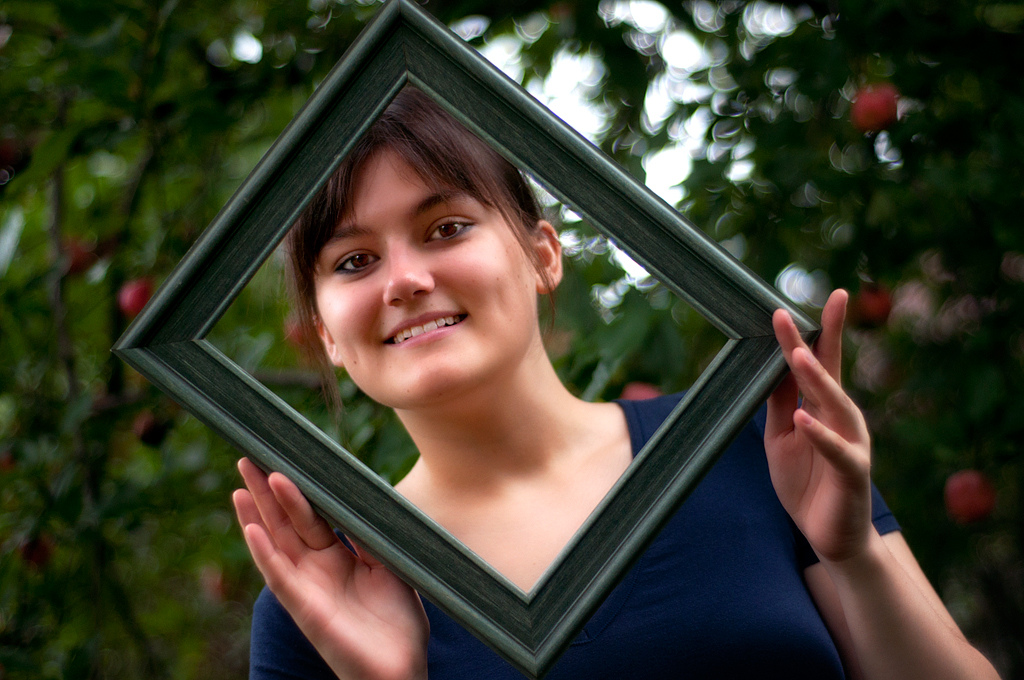
\includegraphics[width=0.9\textwidth]{images/example/example1.png}
	\end{figure}
\end{frame}

\begin{frame}
% example output image
	\frametitle{Example Image}
	\begin{figure}
		\centering
		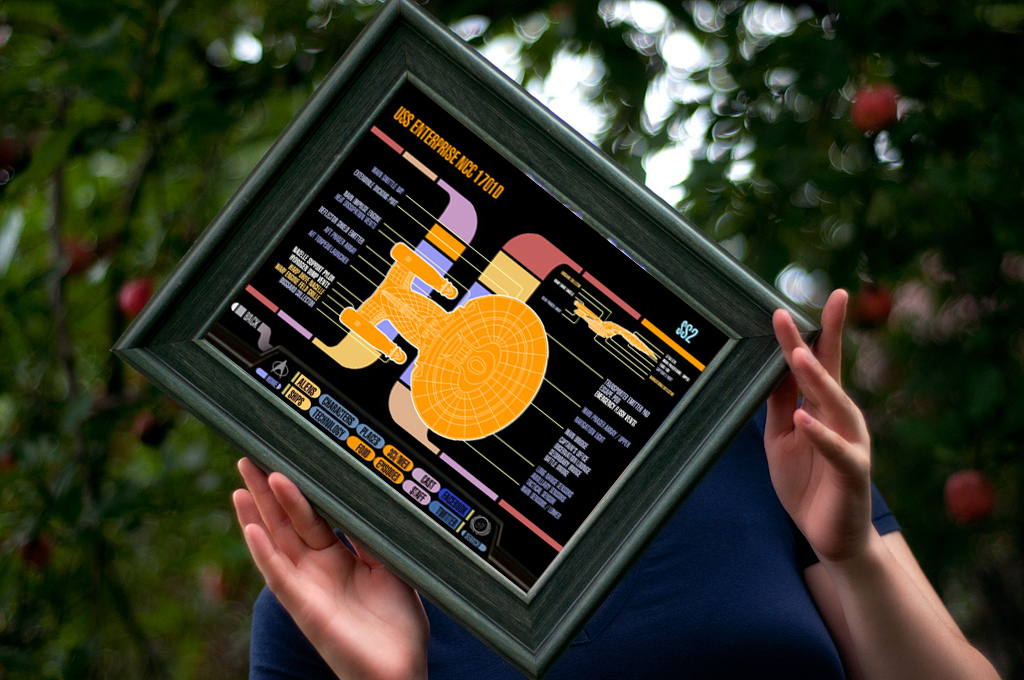
\includegraphics[width=0.9\textwidth]{images/example/example2.jpg}
	\end{figure}
\end{frame}

\begin{frame}
% example output image
	\frametitle{Example Image}
	\begin{figure}
		\centering
		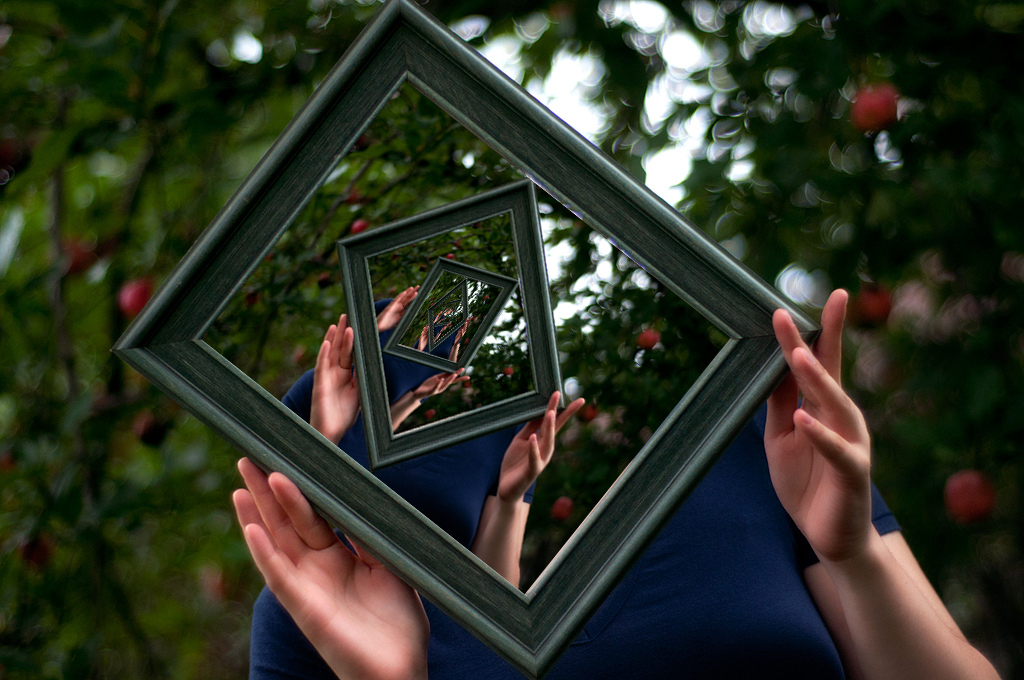
\includegraphics[width=0.9\textwidth]{images/example/example3.jpg}
	\end{figure}
\end{frame}

%Logan
\section{Top-Level Overview}
\begin{frame}
% big block diagram slide
	\frametitle{Top-Level Overview}
	\begin{figure}
		\centering
		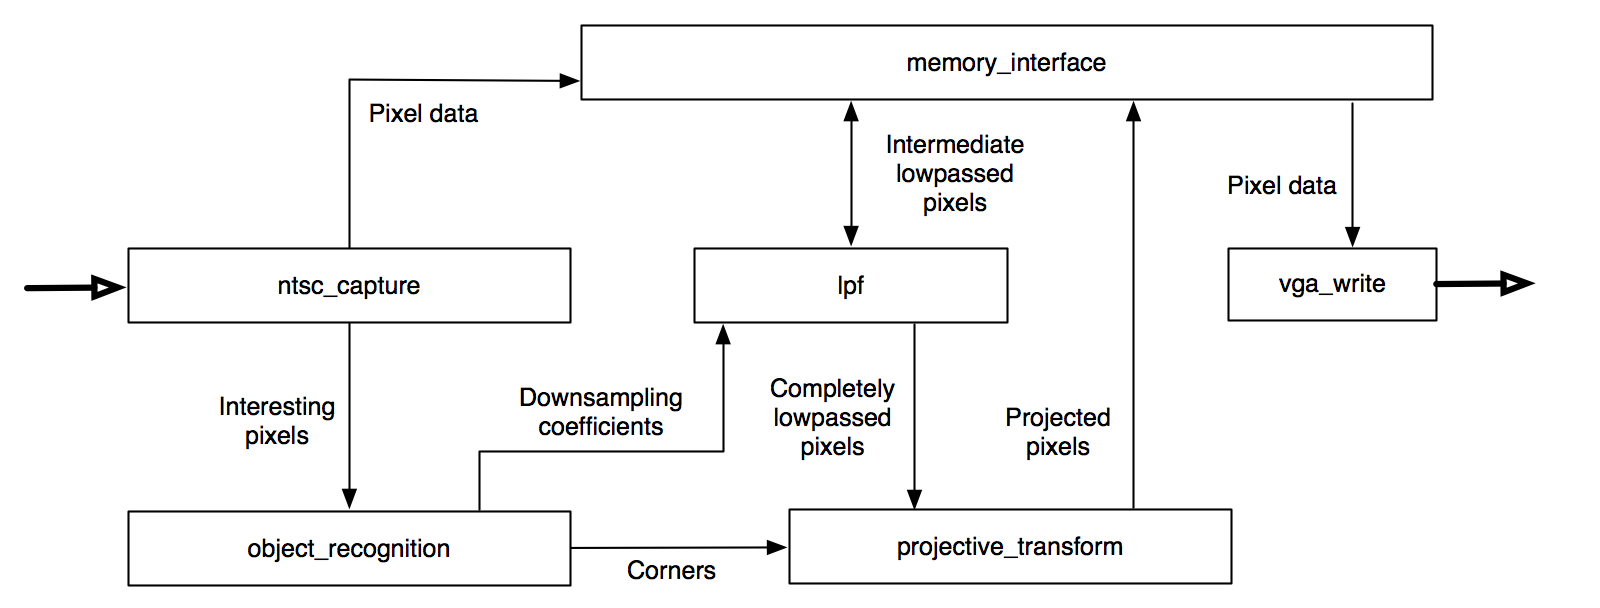
\includegraphics[width=\textwidth]{../proposal/simplified_block_diagram.png}
	\end{figure}
\end{frame}

\section{Individual Module Specifications}
% Logan
\subsection{projective\_transform}
\begin{frame}
	\frametitle{{\tt projective\_transform}: Purpose}
	\begin{figure}
		\centering
		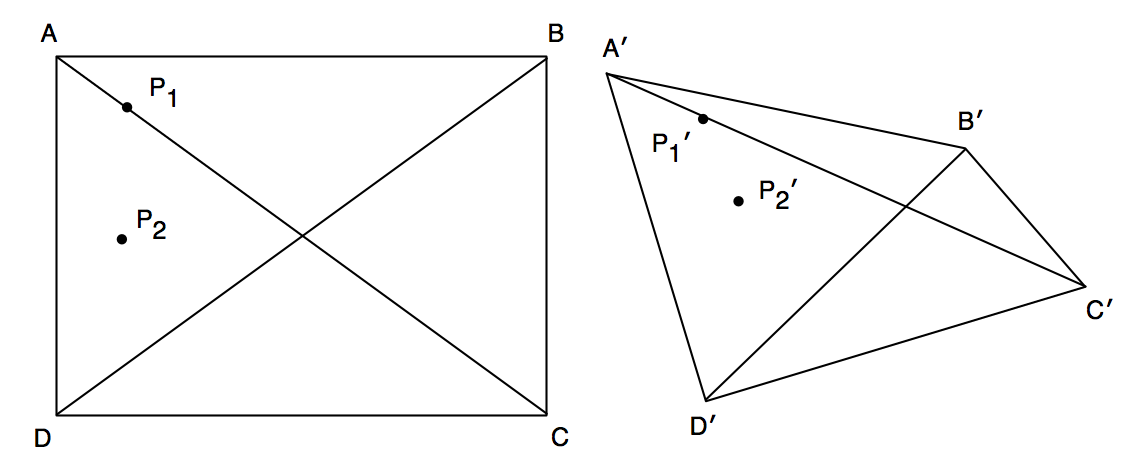
\includegraphics[width=\textwidth]{../proposal/arbiskew_graphic.png}
	\end{figure}
	\begin{itemize}
		\item Skew to any arbitrary convex quadrilateral
	\end{itemize}
\end{frame}

\begin{frame}
	\frametitle{{\tt projective\_transform}: How the algorithm works}
	\begin{figure}
		\centering
		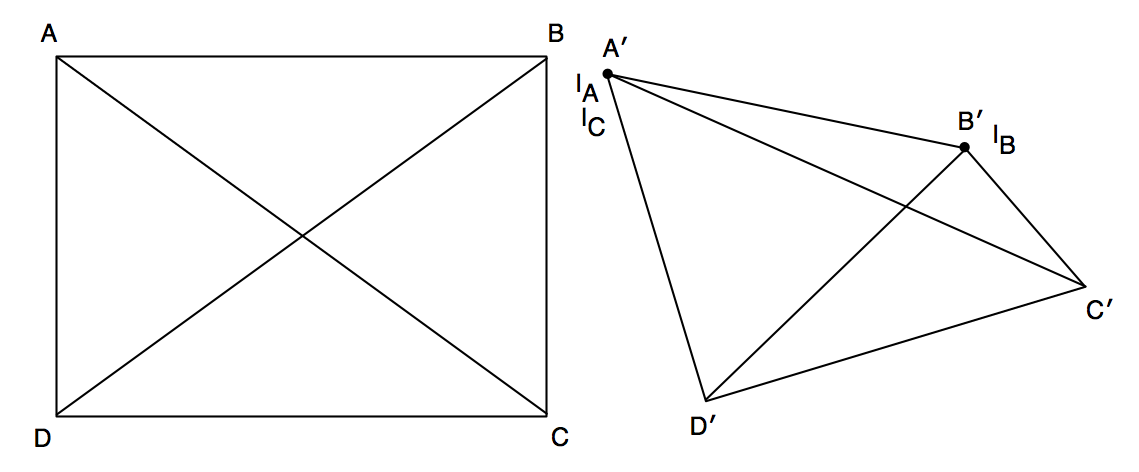
\includegraphics[width=0.7\textwidth]{images/arbiskew_graphic_with_iterators0.png}
	\end{figure}
	\begin{enumerate}
		\item[1]<1-> Calculate the distance of line $\overline{A\prime D\prime}$ and assign it to $d_{ad}$.
		\item[2]<2-> Do the same for $\overline{B\prime C\prime}$ and assign it to $d_{bc}$.
		\item[3]<3-> Create two ``iterator points,'' point $I_A$ and $I_B$ initially located at $A\prime$ and $B\prime$.
		\item[4]<4-> Let $o_x = 0$ and $o_y = 0$
		\item[5]<5-> Calculate the distance between the iterator points, assign it to $d_i$.
		\item[6]<6-> Create a third iterator point, $I_C$ at the location $I_A$.
	\end{enumerate}
\end{frame}

\begin{frame}
	\frametitle{{\tt projective\_transform}: How the algorithm works}
	\begin{figure}
		\centering
		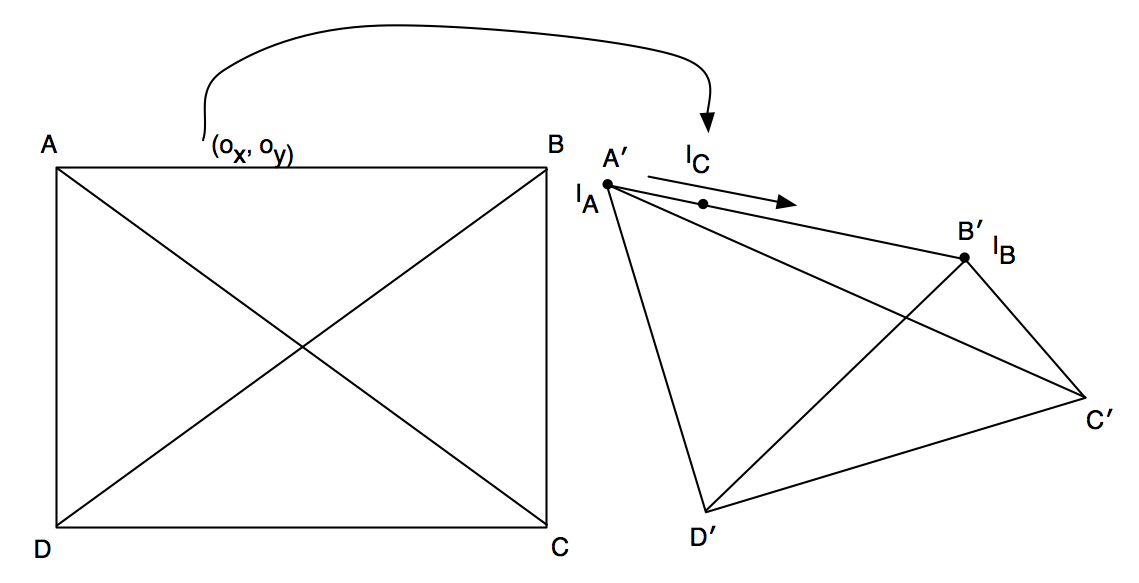
\includegraphics[width=0.7\textwidth]{images/arbiskew_graphic_with_iterators1.png}
	\end{figure}
	\begin{enumerate}
		\item[7]<1-> Assign the pixel value of $I_C$ to pixel $(o_x, o_y)$ in the original image.
		\item[8]<2-> Move $I_C$ along line $\overline{I_A I_B}$ by an amount $= \frac{d_i}{width_{original}}$.
		\item[9]<3-> Increment $o_x$.
		\item[10]<4-> Repeat steps 7--9 until $I_C = I_B$.
	\end{enumerate}
\end{frame}

\begin{frame}
	\frametitle{{\tt projective\_transform}: How the algorithm works}
	\begin{figure}
		\centering
		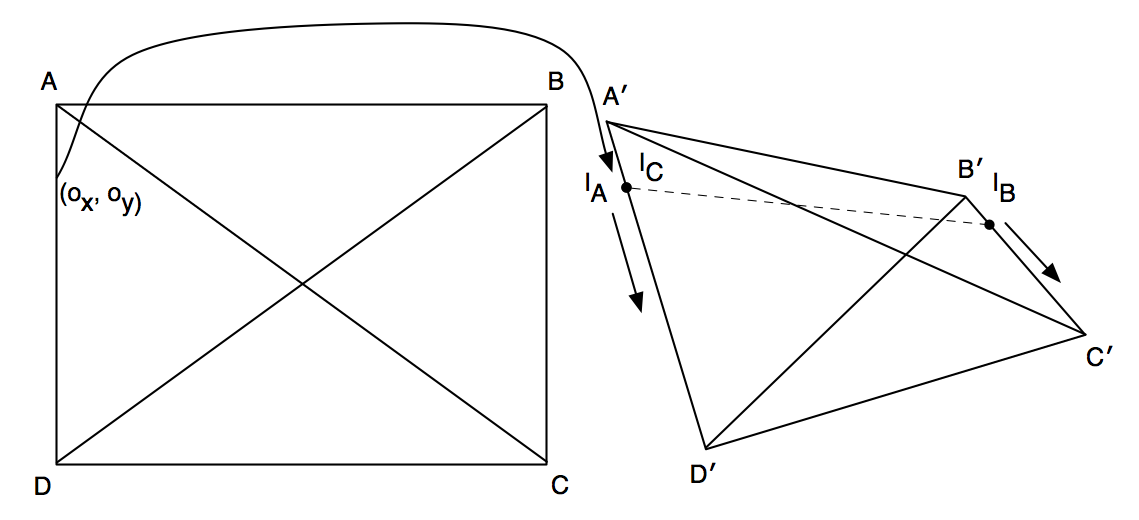
\includegraphics[width=0.7\textwidth]{images/arbiskew_graphic_with_iterators2.png}
	\end{figure}
	\begin{enumerate}
	\item[11]<1-> Move $I_A$ along line $\overline{A\prime D\prime}$ by an amount $= \frac{d_{ad}}{height_{original}}$.
	\item[12]<2-> Move $I_B$ along line $\overline{B\prime C\prime}$ by an amount $= \frac{d_{bc}}{height_{original}}$.
	\item[13]<3-> Increment $o_y$.
	\item[14]<4-> Repeat steps 5--13 until $I_A = D\prime$ and $I_B = C\prime$.
	\end{enumerate}
\end{frame}

\begin{frame}
	\frametitle{{\tt projective\_transform}: How the algorithm works}
	\begin{figure}
		\centering
		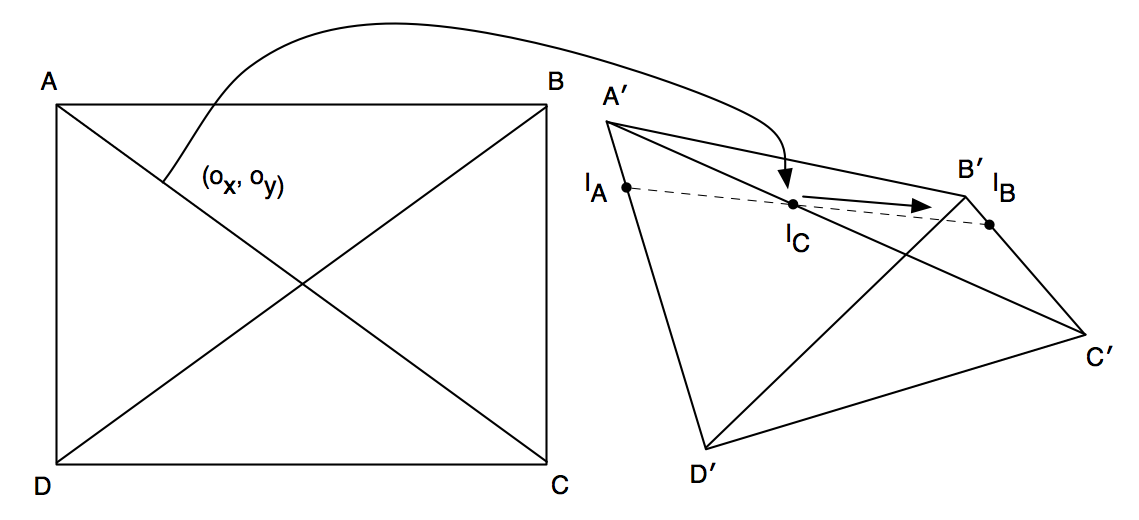
\includegraphics[width=0.7\textwidth]{images/arbiskew_graphic_with_iterators3.png}
	\end{figure}
	\begin{enumerate}
	\item[11] <1->Move $I_A$ along line $\overline{A\prime D\prime}$ by an amount $= \frac{d_{ad}}{height_{original}}$.
	\item[12] Move $I_B$ along line $\overline{B\prime C\prime}$ by an amount $= \frac{d_{bc}}{height_{original}}$.
	\item[13] Increment $o_y$.
	\item[14] Repeat steps 5--13 until $I_A = D\prime$ and $I_B = C\prime$.
	\end{enumerate}
\end{frame}

\begin{frame}
	\frametitle{{\tt projective\_transform}: Example}
	\begin{figure}
		\centering
		\includegraphics[width=0.8\textwidth]{../../sketches/arbiskew/IMG_5046.jpg}
		\caption{The original image}
	\end{figure}
\end{frame}

\begin{frame}
	\frametitle{{\tt projective\_transform}: Example}
	\begin{figure}
		\centering
		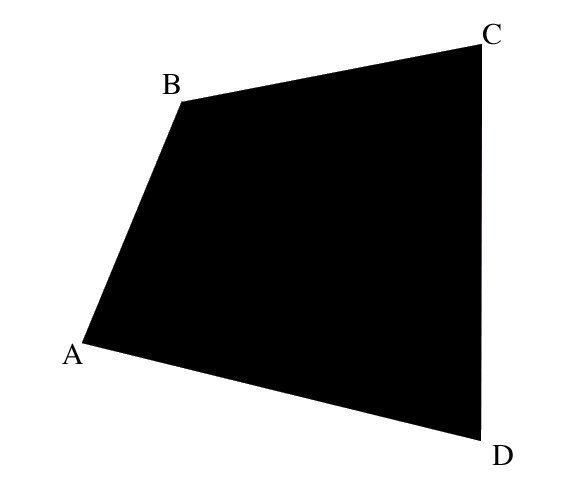
\includegraphics[width=0.8\textwidth]{images/skew_example/skew_rectangle.png}
		\caption{We want it skewed to this quadrilateral}
	\end{figure}
\end{frame}

\begin{frame}
	\frametitle{{\tt projective\_transform}: Example}
	\begin{figure}
		\centering
		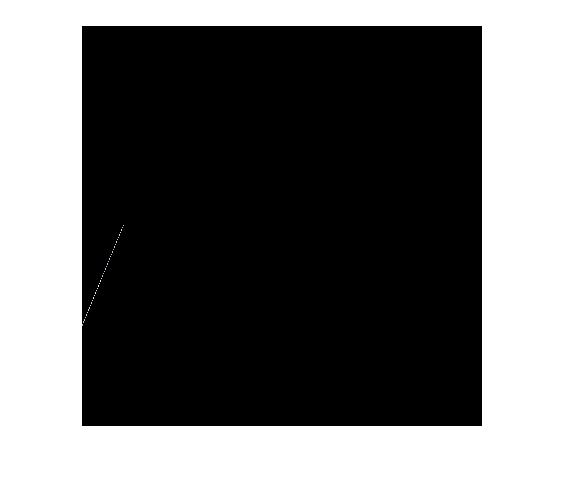
\includegraphics[width=0.8\textwidth]{images/skew_example/projected_halfway_line.jpg}
		\caption{Halfway along line $A\prime B\prime$}
	\end{figure}
\end{frame}

\begin{frame}
	\frametitle{{\tt projective\_transform}: Example}
	\begin{figure}
		\centering
		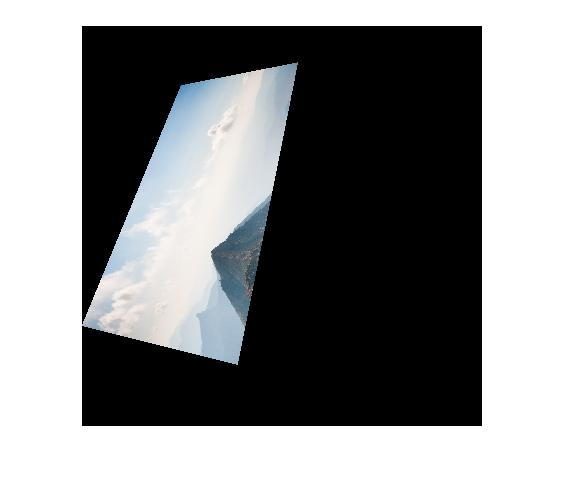
\includegraphics[width=0.8\textwidth]{images/skew_example/projected_halfway.jpg}
		\caption{Halfway through skewing the image}
	\end{figure}
\end{frame}

\begin{frame}
	\frametitle{{\tt projective\_transform}: Example}
	\begin{figure}
		\centering
		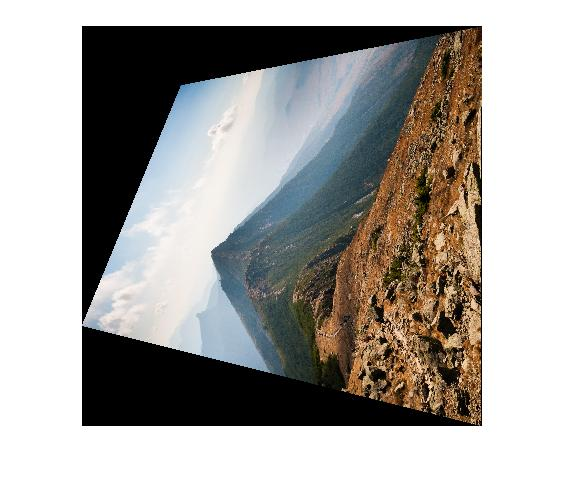
\includegraphics[width=0.8\textwidth]{images/skew_example/projected_final.jpg}
		\caption{The final image (processed with MATLAB)}
	\end{figure}
\end{frame}

\begin{frame}
	\frametitle{{\tt projective\_transform}: FPGA implementation}
	\begin{itemize}
	\item<1-> Straightfoward state based implementation of the above algorithm
	\item<2-> Requires $2\times640\times480 + 4\times480 \approx 2\times640\times480 = 614,400$ multiplications per frame cycle
	\item<3-> Uses coregen Divider modules for the divisions
	\item<4-> Uses an iterative algorithm for finding distances (pipelined at the end of each line of the image)
	\item<5-> Processes pixels ``on-the-fly'' from {\tt LPF}
	\item<6-> Negligible BRAM memory requirements (a handful of registers)
	\end{itemize}
\end{frame}


\begin{frame}
	\frametitle{{\tt projective\_transform}: How it Interfaces}
	\begin{figure}
		\centering
		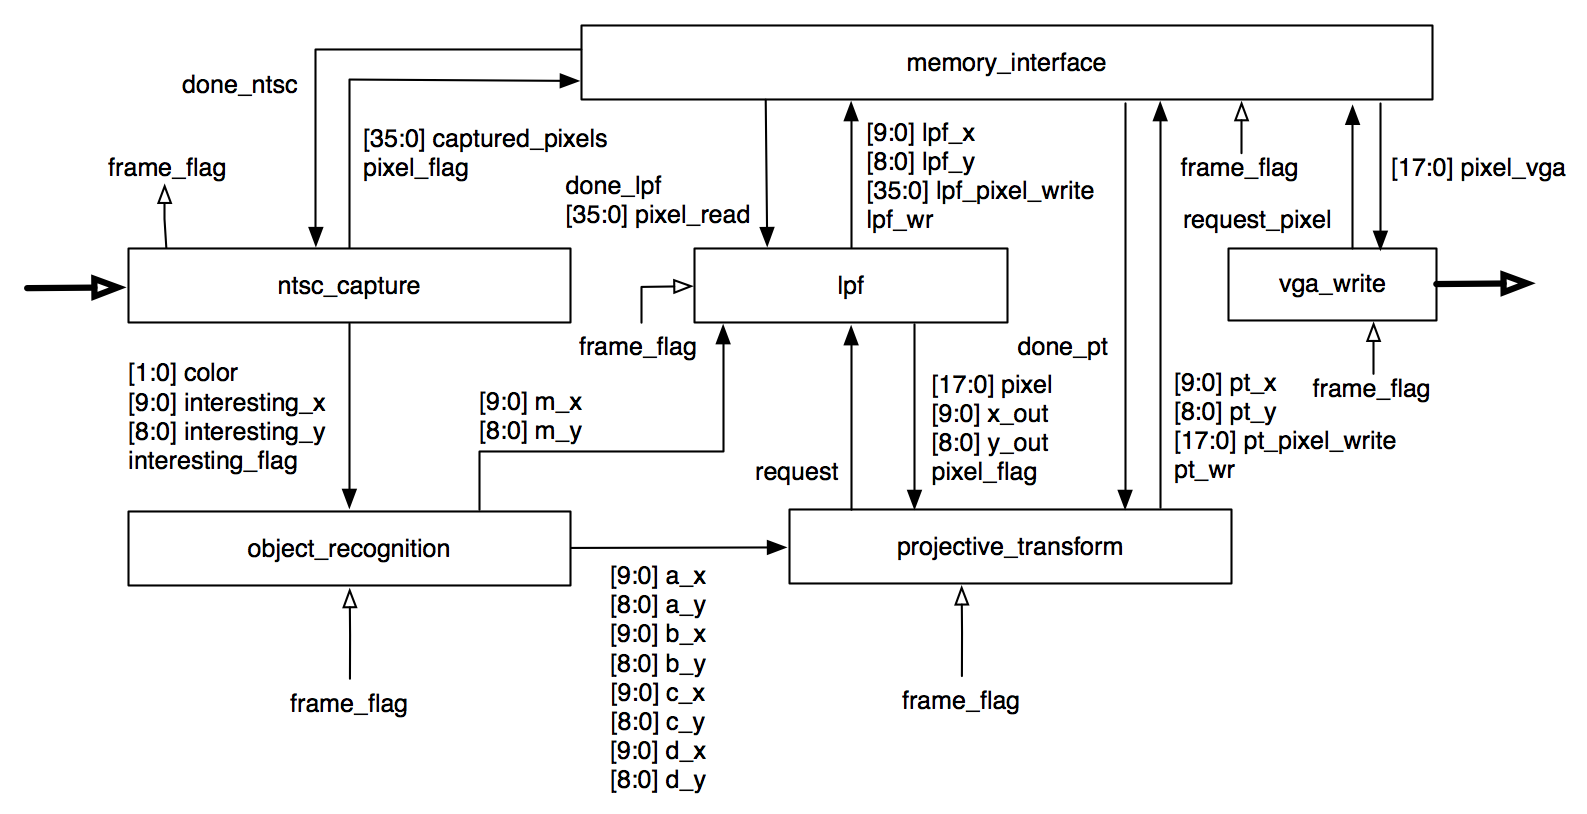
\includegraphics[width=\textwidth]{../proposal/block_diagram_with_wires.png}
	\end{figure}
\end{frame}

% Logan
\subsection{object\_recognition}


\begin{frame}
	\frametitle{{\tt object\_recognition}}

	\begin{figure}
		\centering
		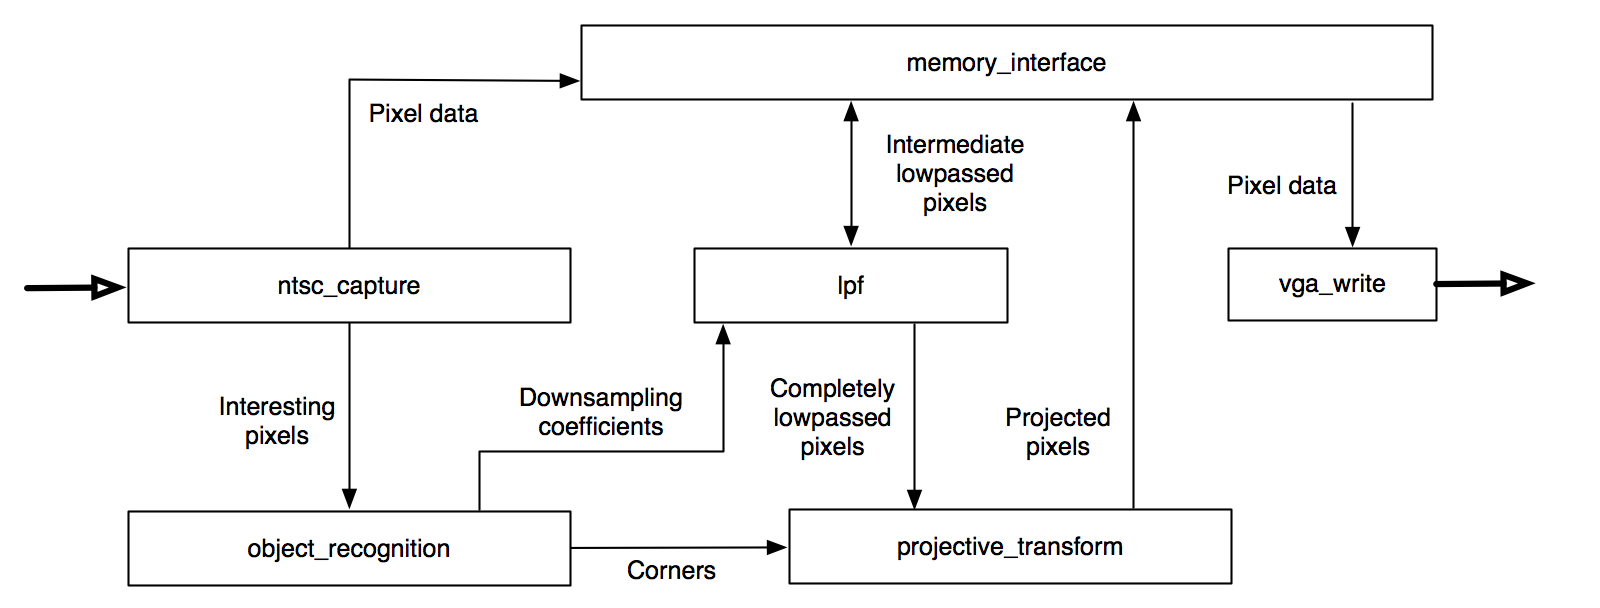
\includegraphics[width=0.8\textwidth]{../proposal/simplified_block_diagram.png}
	\end{figure}
	
	\begin{itemize}
		\item Mark corners of frame with four differently colored dots.
		\item Recognition begins in the {\tt ntsc\_capture} module, which detects these colors as it is capturing data and sends the pixel info to the {\tt object\_recognition} module.
		
	\end{itemize}
\end{frame}

\begin{frame}
	\frametitle{{\tt object\_recognition}}

	\begin{itemize}
		\item Take linear weighted center of mass for each color
		\item Sums the (x,y) coordinates for each color as it receives them. (8 running sums, 2 for each color)
		\item When the frame is done, divide each sum by the number of summed items
		\item The resulting 4 (x,y) pairs are the corners of the frame
		\item By looking for pixels in {\tt ntsc\_capture} we significantly reduce the amount of time spent in {\tt object\_recognition}
	\end{itemize}
\end{frame}

% Jose
\subsection{LPF}
\begin{frame}
	\frametitle{{\tt LPF}: its purpose}
	\begin{columns}[c]
		\column{.5\textwidth}
		\begin{itemize}
		\item<1-> {\tt projective\_transform} \(\rightarrow\) aliasing
		\item<2-> Aliasing reduces the quality of an image
		\item<3-> Lowpass filtering prevents aliasing
		\item<6-> Information of an image is mostly phase
		\item<7-> Symmetric Type I FIR filter \(\rightarrow\) 0 phase distortion
		\item<8-> Parks-McClellan: reasonable accuracy, symmetric, easily calculable
		\item<9-> FIR PM filter reduces mem. acceses to 1.5/pixel
		\end{itemize}
	
		\column{.5\textwidth}
		\begin{figure}
			\centering
			\uncover<1->{\subfigure[Original]{\includegraphics[width=0.4\textwidth]{images/lpf/lpf-purpose/original.png}}}
			\uncover<2-3,5->{\subfigure[Aliased]{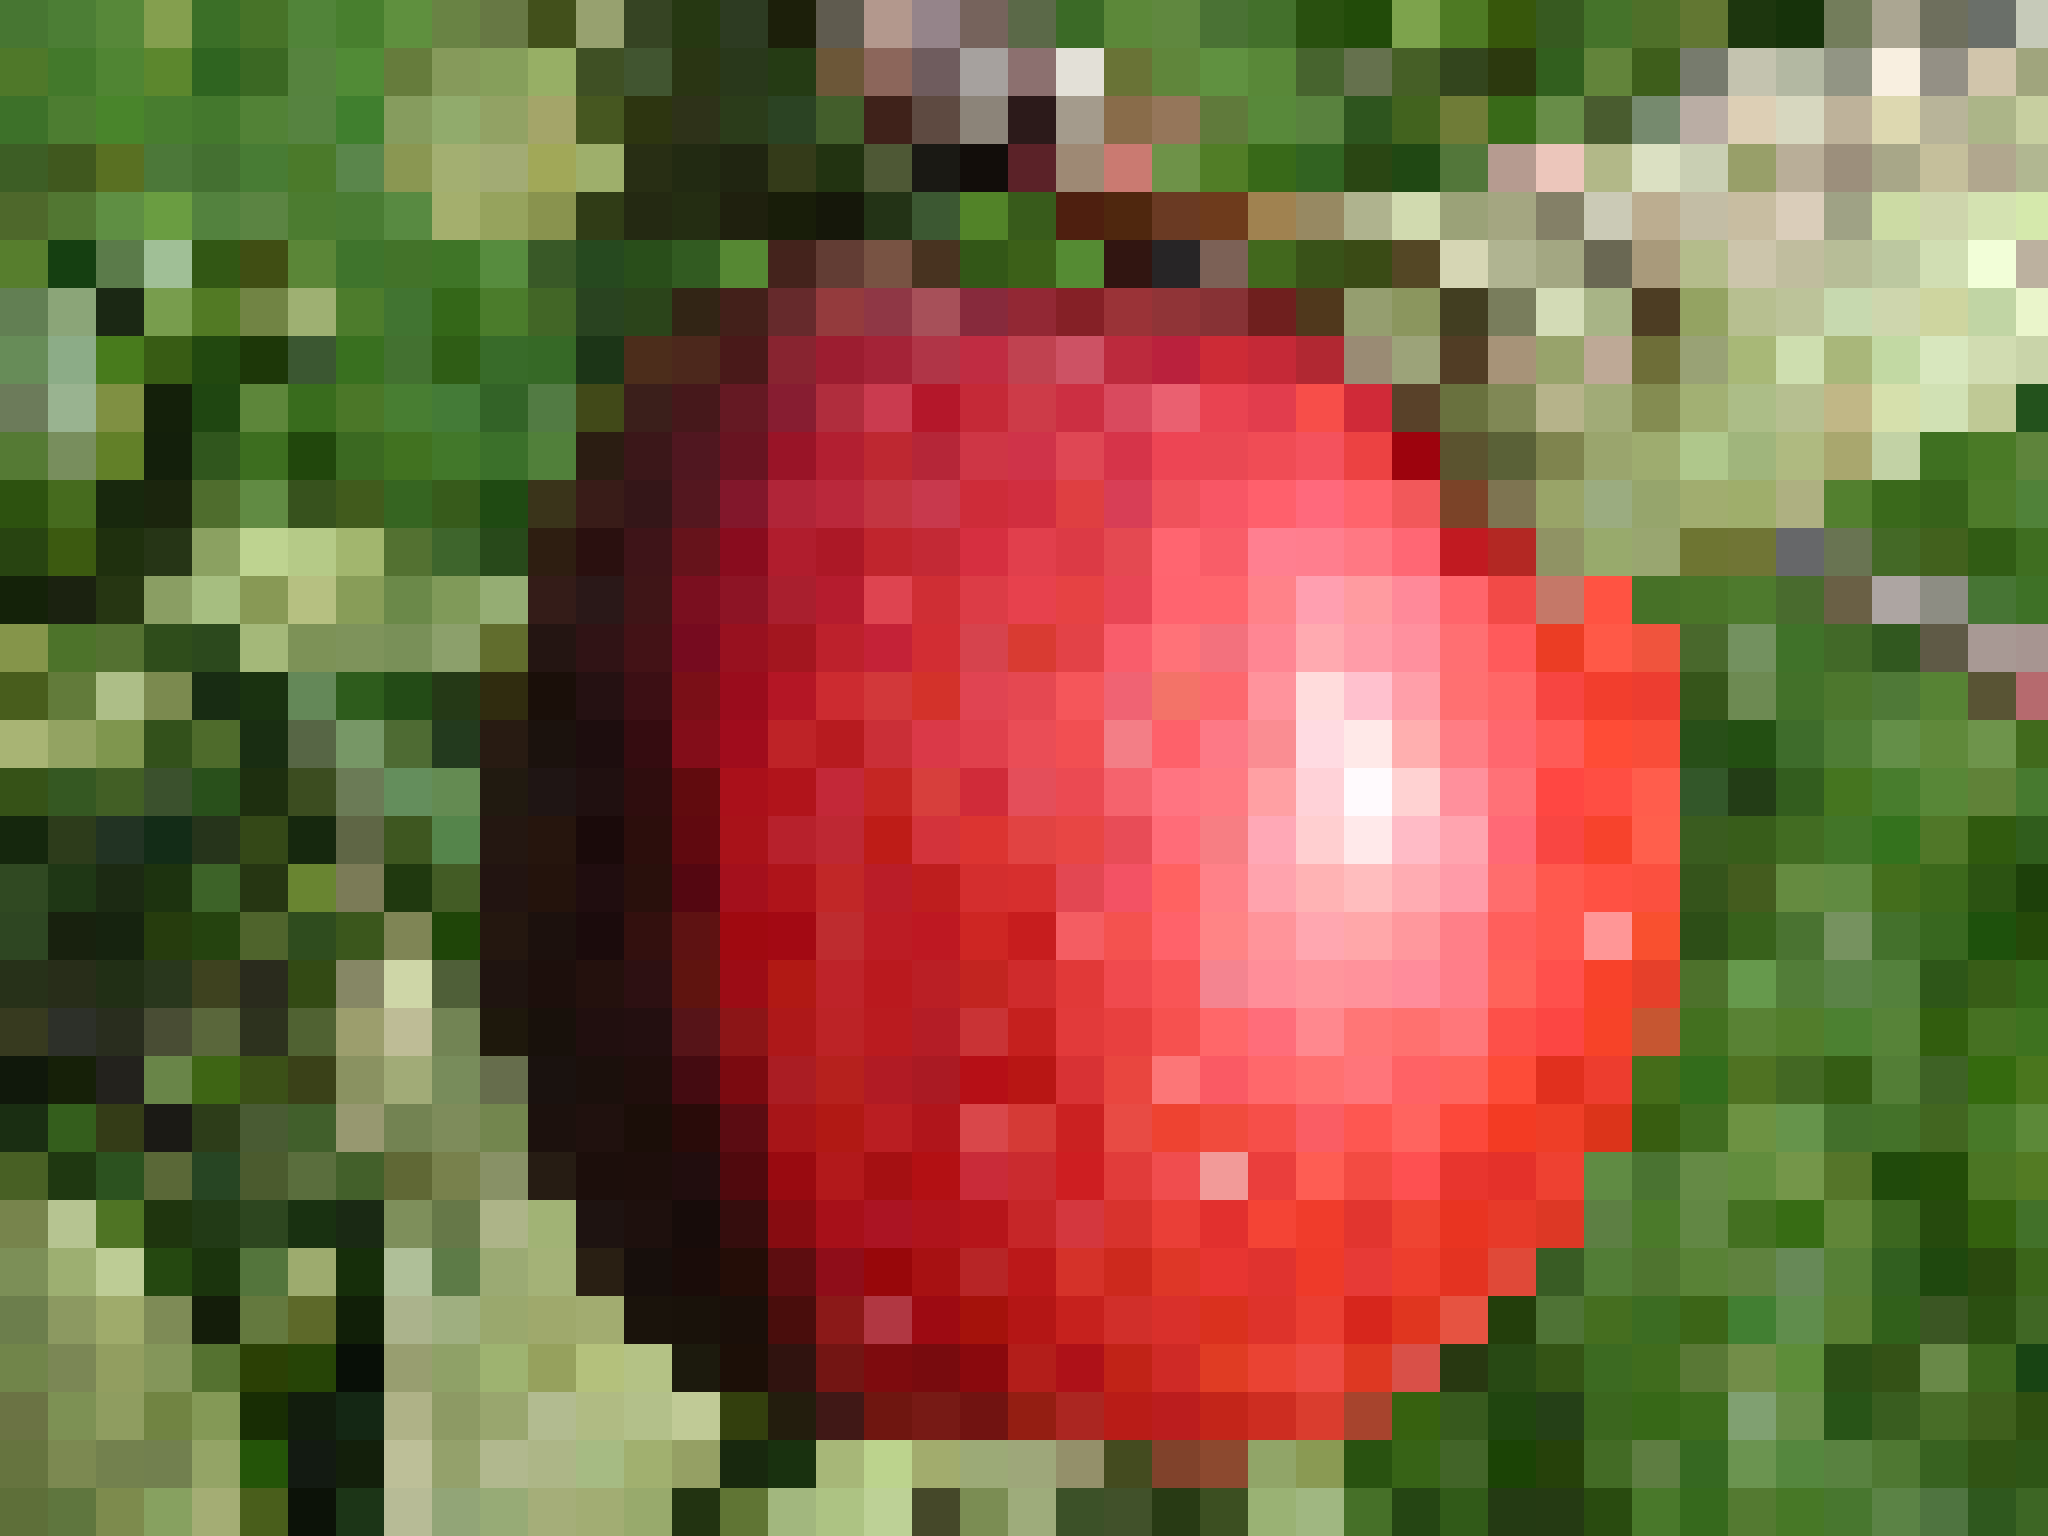
\includegraphics[width=0.4\textwidth]{images/lpf/lpf-purpose/original_aliased.png}}}
		\end{figure}
		\begin{figure}
			\centering
			\uncover<3->{\subfigure[Mag. of Filter]{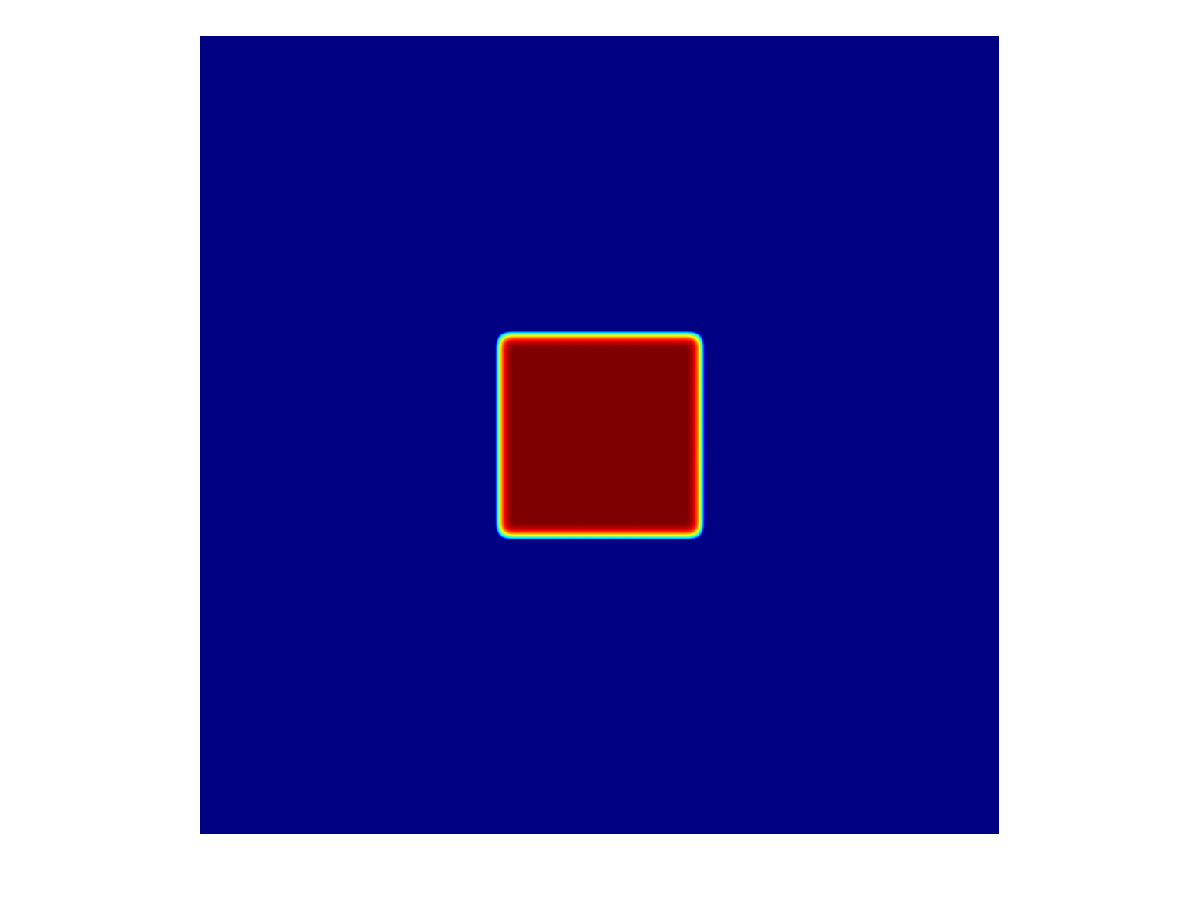
\includegraphics[width=0.4\textwidth]{images/lpf/lpf-purpose/filter_mag.png}}}
			\uncover<4->{\subfigure[Filtered]{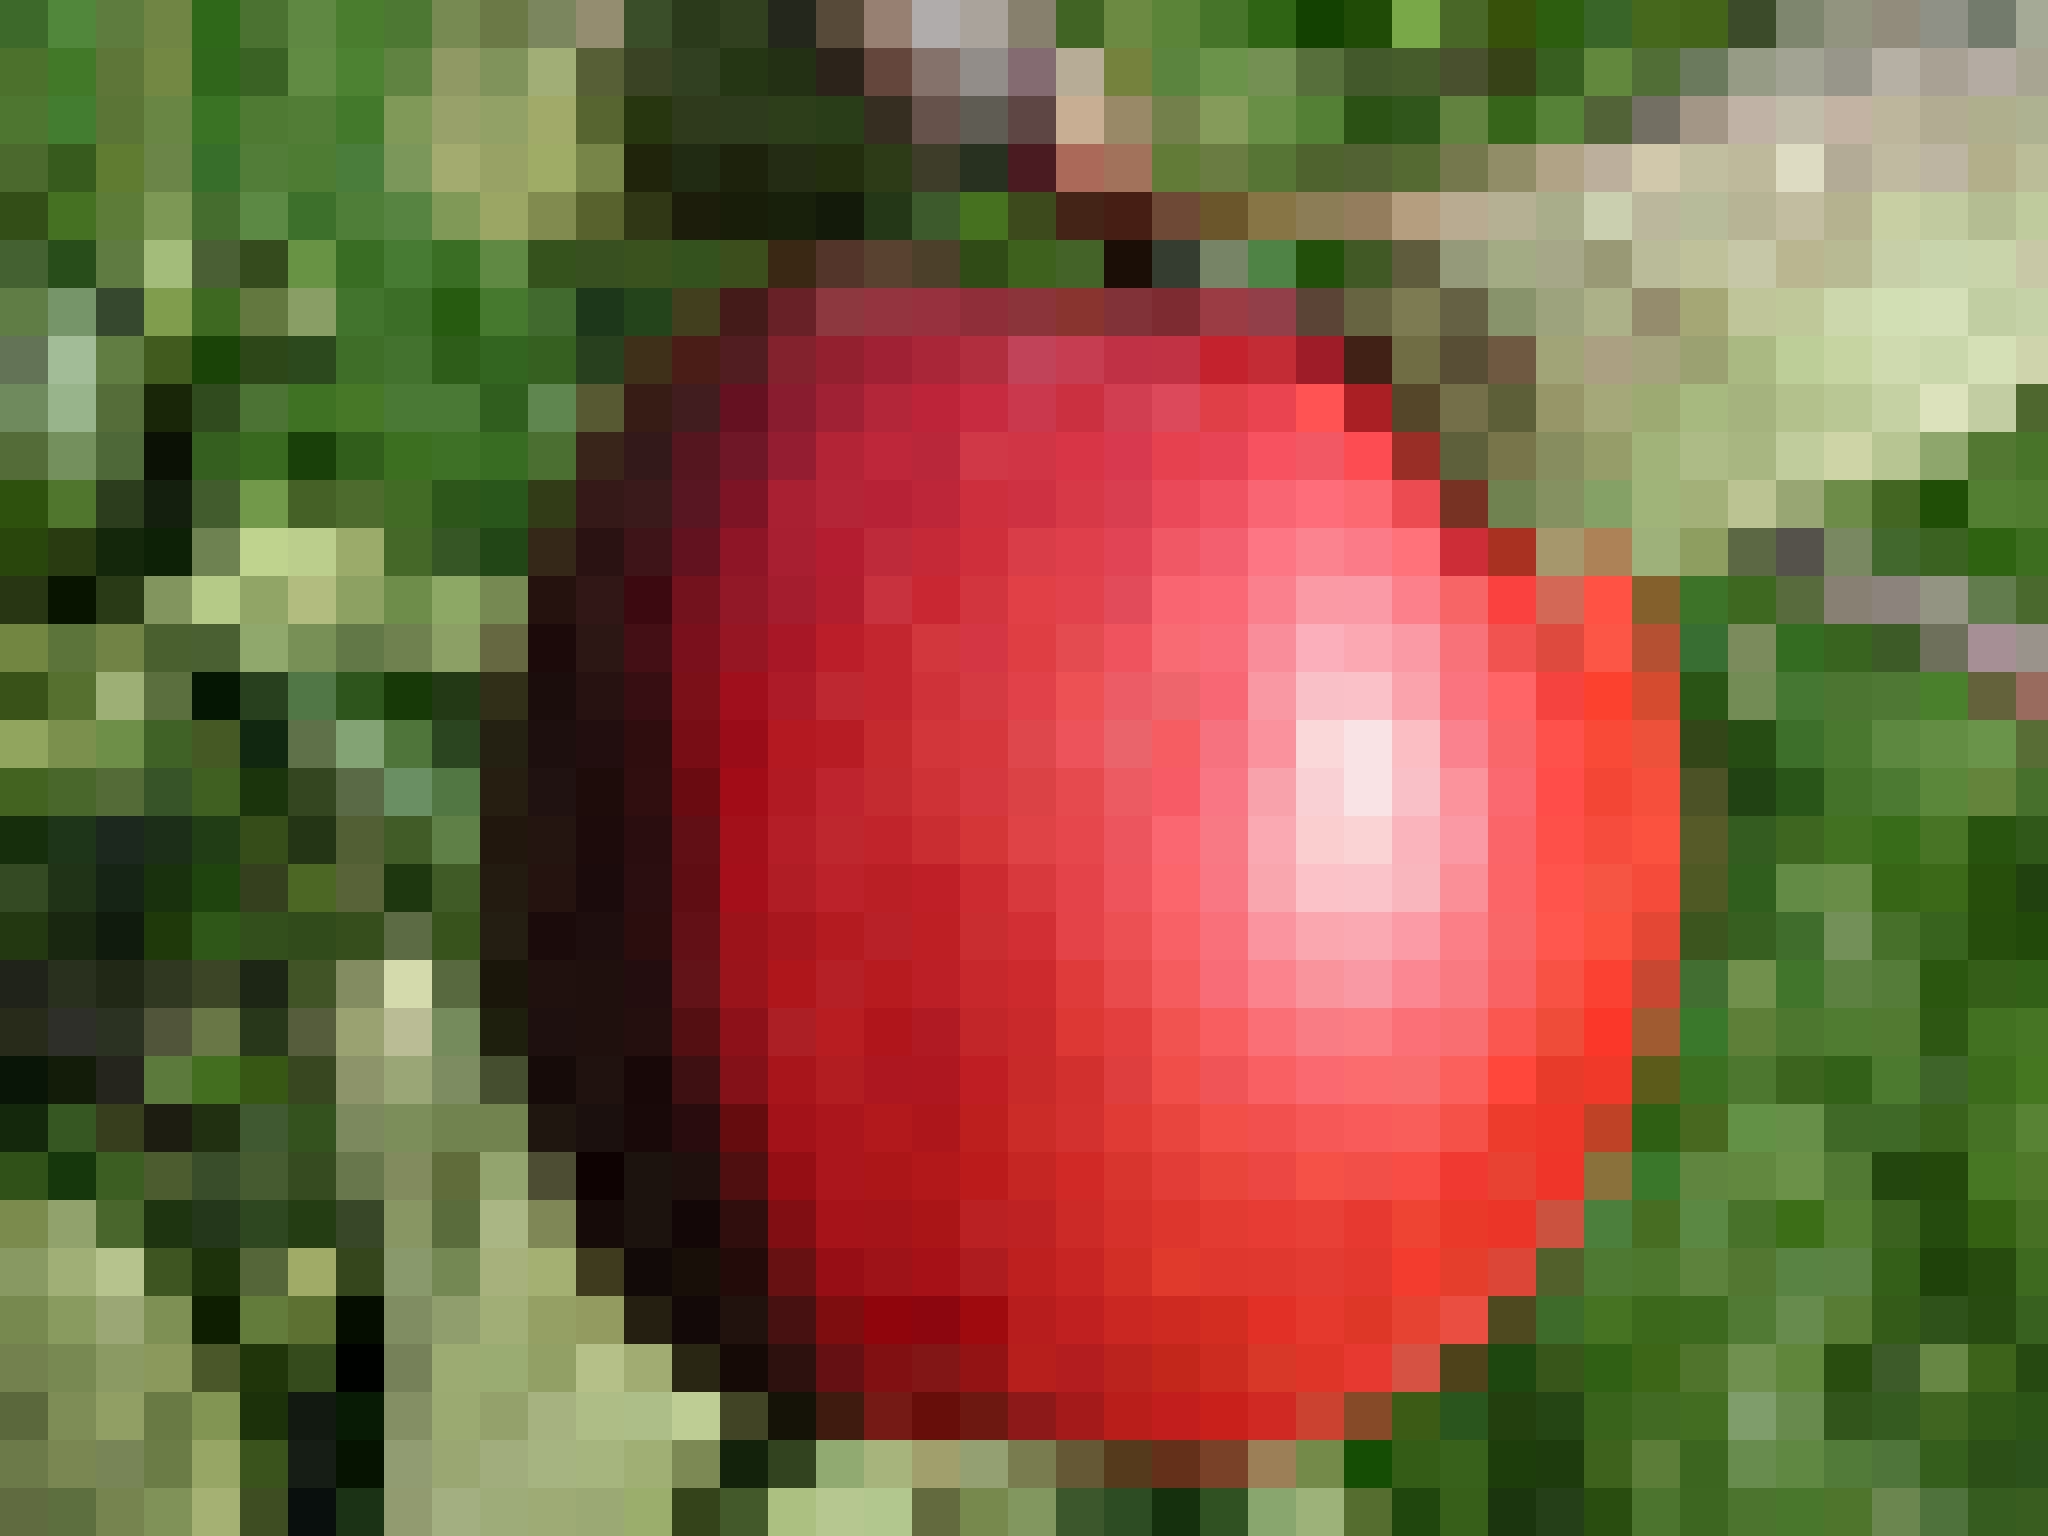
\includegraphics[width=0.4\textwidth]{images/lpf/lpf-purpose/original_filtered.png}}}
		\end{figure}
	\end{columns}
\end{frame}
\begin{frame}
	\frametitle{{\tt LPF}: the algorithm}
	\begin{columns}[t]
		\column{.5\textwidth}
		\begin{enumerate}
		\item<1-> Given an arbitrary image \& skewing coefficients \( M_x \) \& \( M_y \).
		\item<2-> Fetch a filter with cutoff \( \frac{\pi}{M_y} \).
		\item<3-> Filter each column and store in memory.
		\item<4-> Fetch a filter with cutoff \( \frac{\pi}{M_x} \).
		\item<5-> Filter each row and output to {\tt projective\_transform}.
		\item<6-> Repeat this process every refresh cycle.
		\end{enumerate}

		\column{.5\textwidth}
		\begin{figure}
			\centering
			\only<1>{\subfigure[F.T. Original]{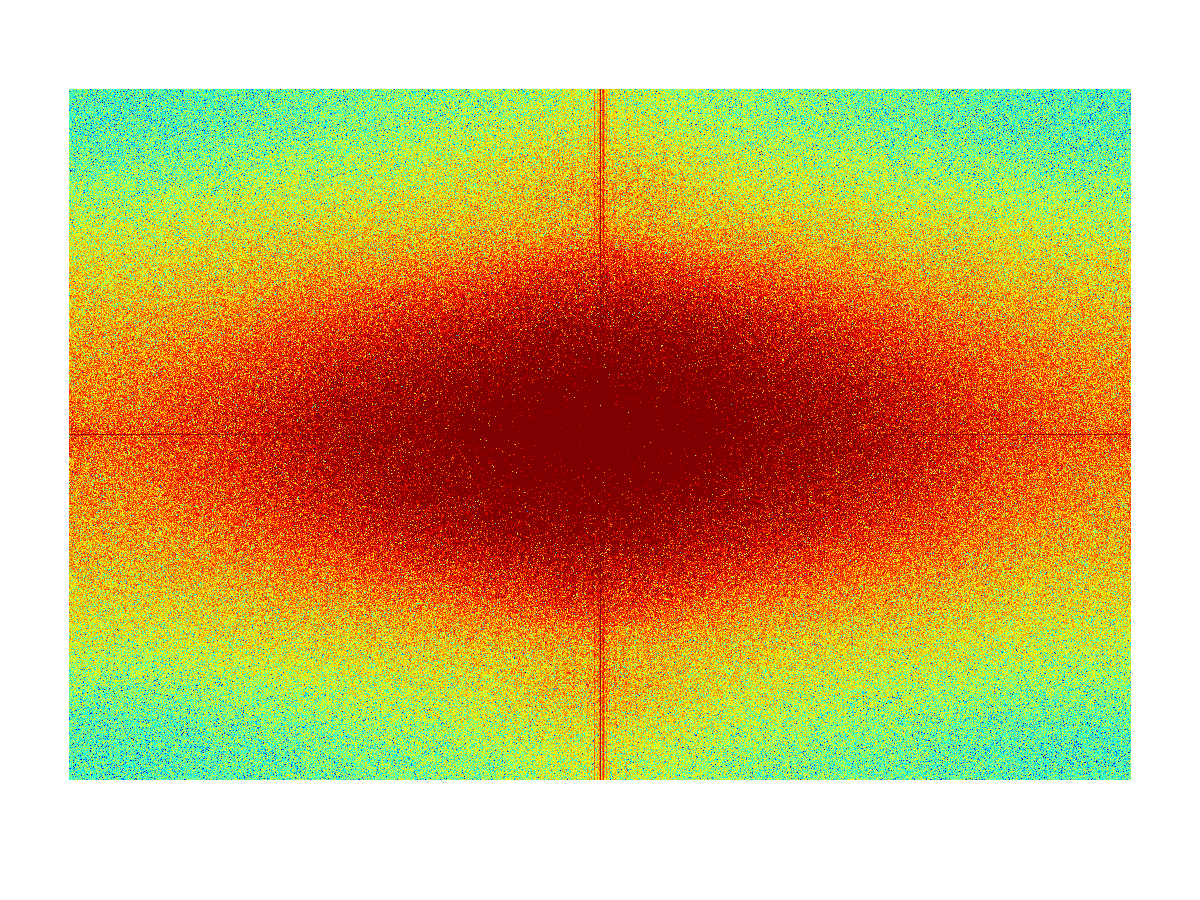
\includegraphics[width=0.45\textwidth]{images/lpf/lpf-operation/orig_mag.png}}\subfigure[Original Image]{\includegraphics[width=0.45\textwidth]{images/lpf/lpf-operation/original.jpg}}}
			\only<2-3>{\subfigure[F.T. Original]{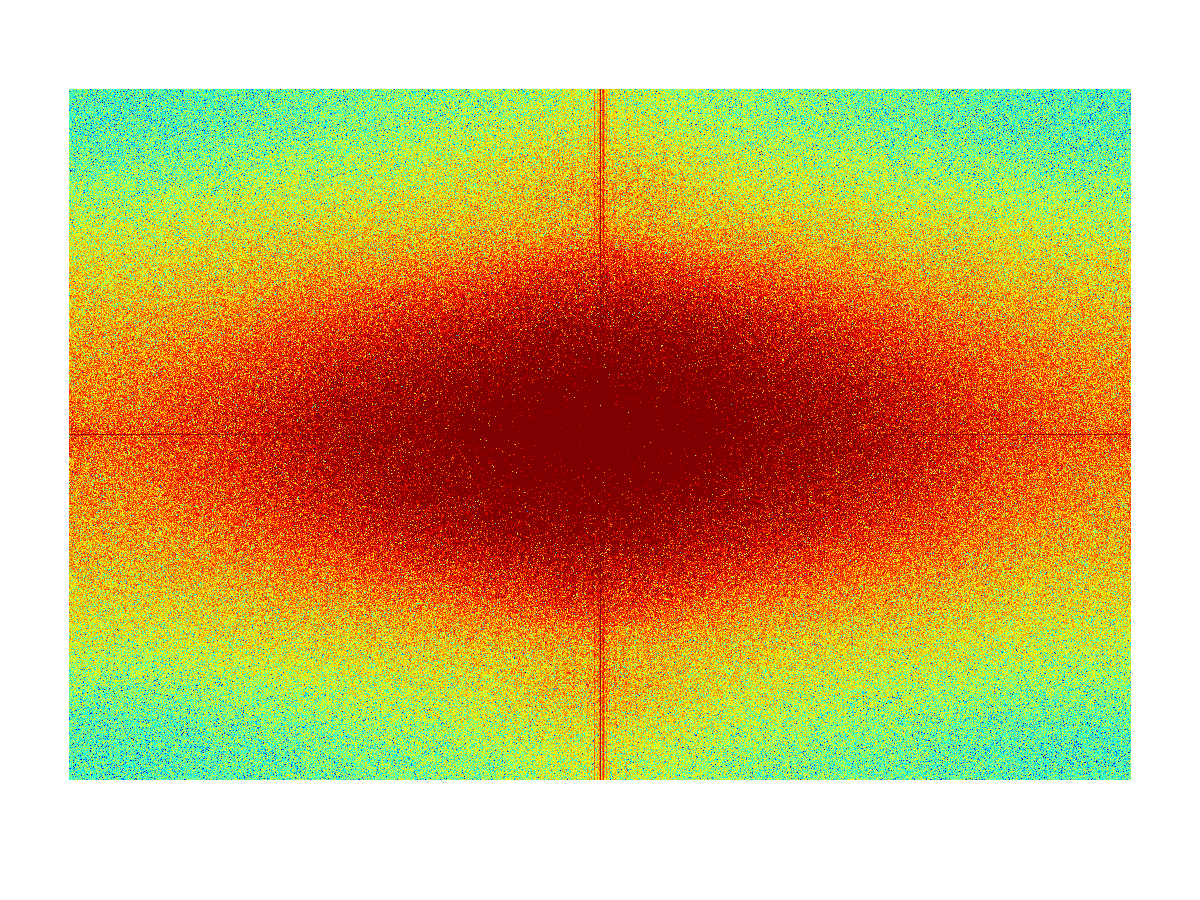
\includegraphics[width=0.45\textwidth]{images/lpf/lpf-operation/orig_mag.png}}\subfigure[1D FIR, $\omega_c=\frac{\pi}{8}$]{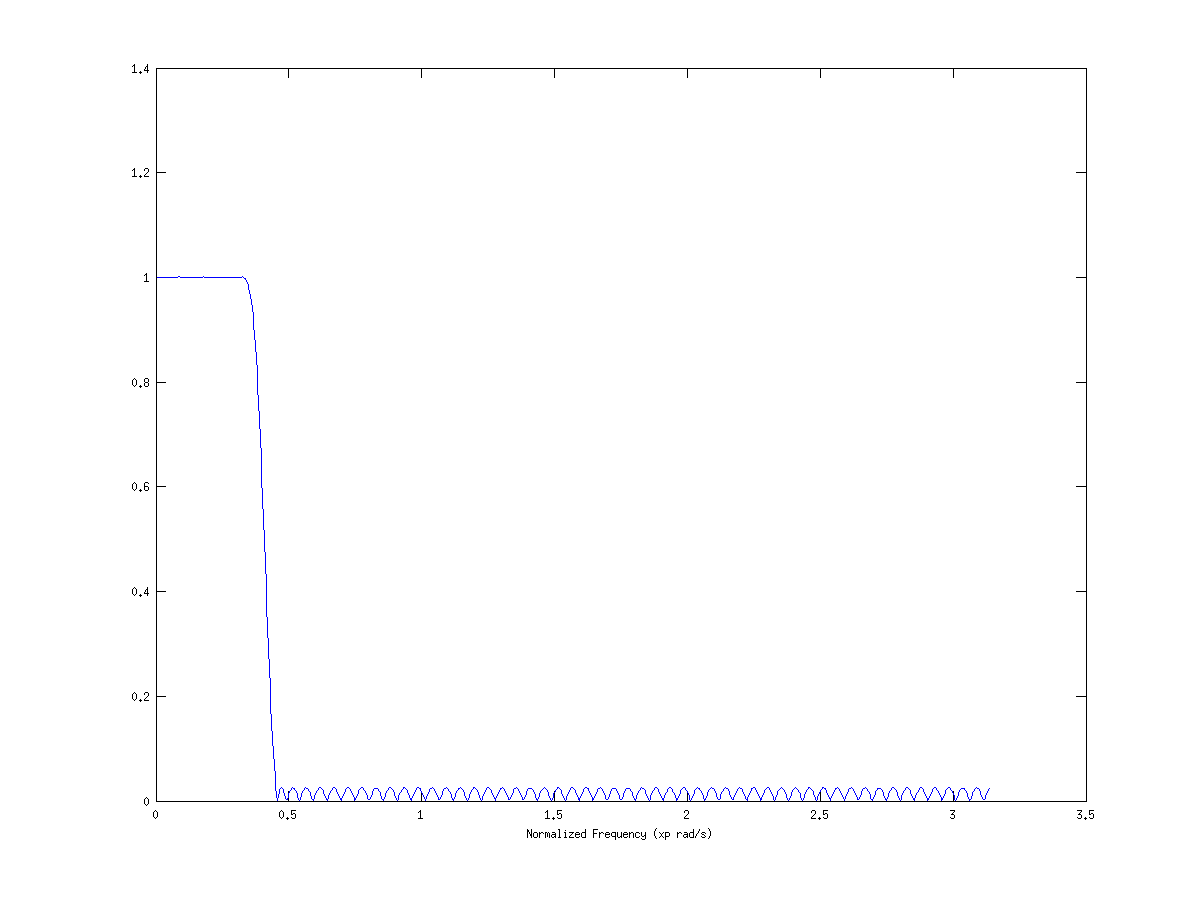
\includegraphics[width=0.45\textwidth]{images/lpf/lpf-operation/y-filter.png}}}
			\only<4-5>{\subfigure[F.T. Filtered]{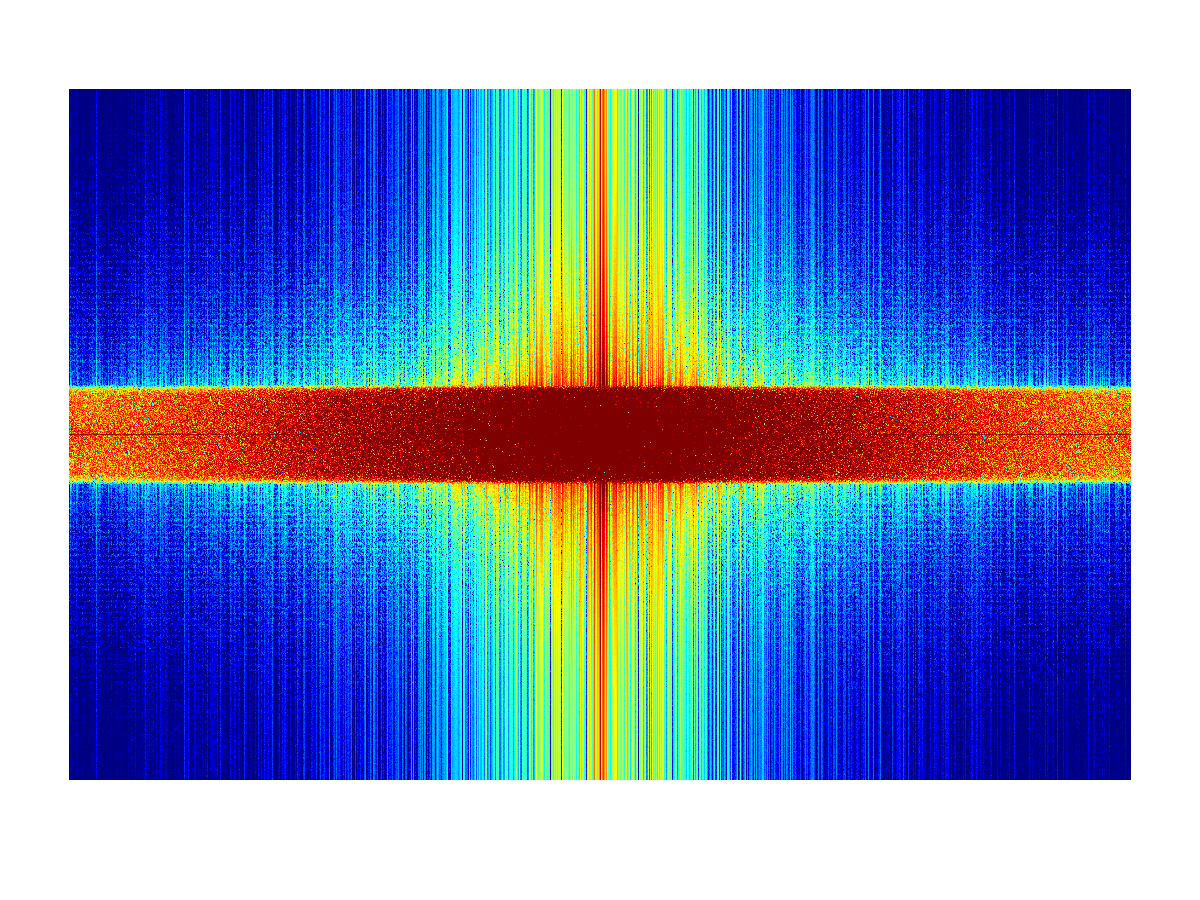
\includegraphics[width=0.45\textwidth]{images/lpf/lpf-operation/proc_mag.png}}\subfigure[1D FIR, $\omega_c=\frac{\pi}{16}$]{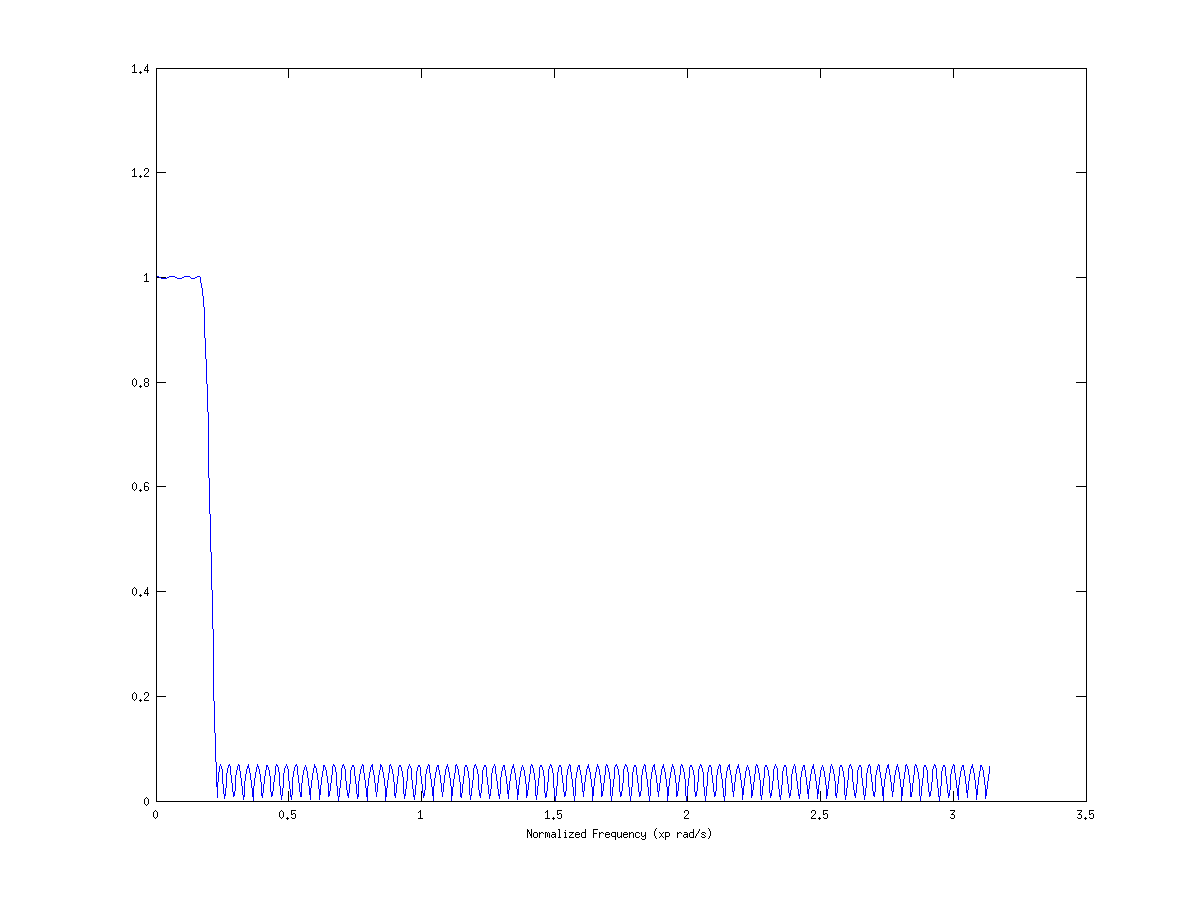
\includegraphics[width=0.45\textwidth]{images/lpf/lpf-operation/x-filter.png}}}
			\only<6>{\subfigure[Original]{\includegraphics[width=0.45\textwidth]{images/lpf/lpf-operation/original.jpg}}\subfigure[F.T. of Process]{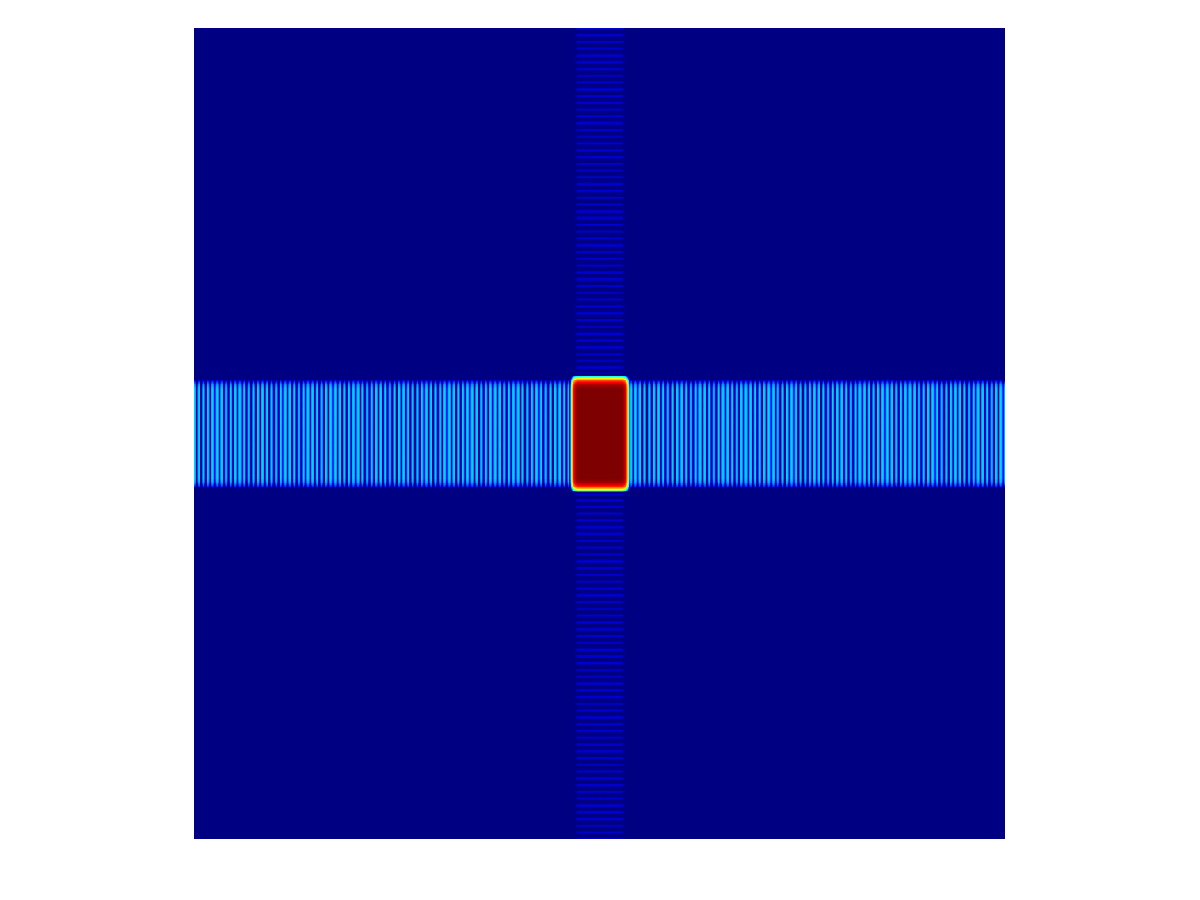
\includegraphics[width=0.4\textwidth]{images/lpf/lpf-operation/total_filt.png}}}
		\end{figure}

		\begin{figure}
			\only<3>{\subfigure[F.T. Filtered]{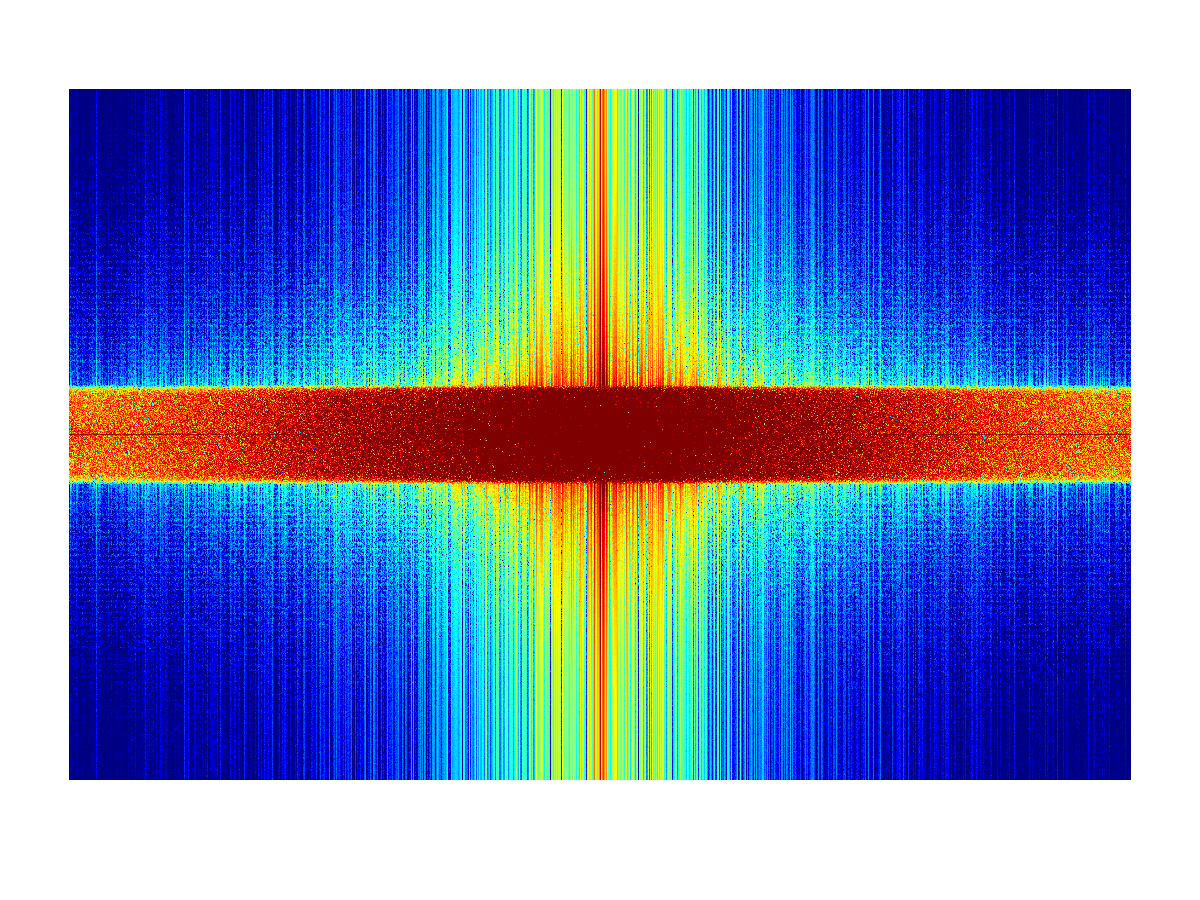
\includegraphics[width=0.4\textwidth]{images/lpf/lpf-operation/proc_mag.png}}}
			\only<5>{\subfigure[F.T. Output]{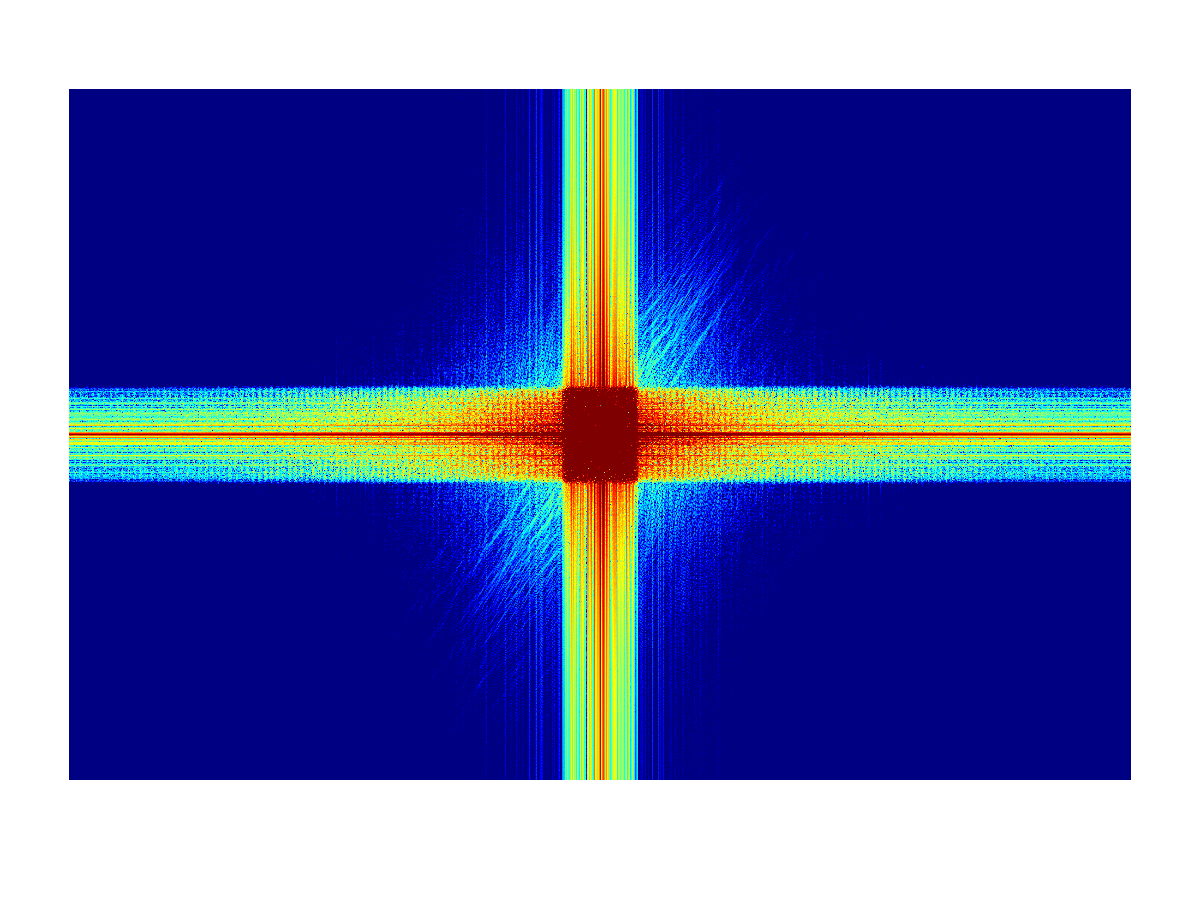
\includegraphics[width=0.4\textwidth]{images/lpf/lpf-operation/output_mag.png}}}
			\only<6>{\subfigure[Output]{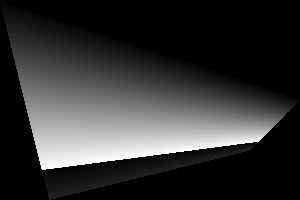
\includegraphics[width=0.4\textwidth]{images/lpf/lpf-operation/output.png}}}
		\end{figure}

	\end{columns}
\end{frame}

% Jose
\subsection{memory\_interface}
\begin{frame}
	\frametitle{{\tt memory\_interface}}
	\begin{columns}[t]
		\column{.6\textwidth}
		\begin{itemize}
		\item<1-> 1 image is a lot of data: \( 640\cdot480\cdot24 \text{ bits} \approx 0.88 \text{MiB} \)
		\item<2-> Total BRAM: \( 0.316 \text{MiB} \)
		\item<3-> We need to store 4 images in memory!
		\item<4-> Let's use the ZBT RAM: \( 2\cdot2.25 \text{MiB} \)
		\item<5-> Not so fast: 1 clock cycle per memory access
		\item<6-> 1 pixel per address would require a clock speed \( > 100MHz \)
		\item<7-> Let's store store 18 bits per pixel or 2 per address
		\end{itemize}

		\column{.4\textwidth}
	\end{columns}
\end{frame}

\begin{frame}
	\frametitle{{\tt memory\_interface}: operation}
	\begin{center}
		Four images in memory:
	\end{center}
	\begin{figure}
		\centering
		\uncover<1->{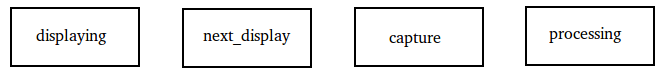
\includegraphics[width=0.8\textwidth]{images/memory_interface/before_shift.png}}
		\uncover<2->{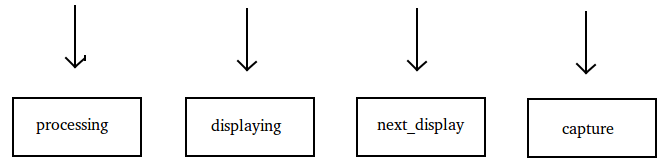
\includegraphics[width=0.8\textwidth]{images/memory_interface/after_shift.png}}
	\end{figure}
	\begin{center}
		\uncover<2->{Shift every refresh cycle}
	\end{center}
\end{frame}

% Jose
\subsection{system io}
\begin{frame}
	\frametitle{system io: {\tt ntsc\_capture} \& {\tt vga\_write}}
	%\begin{columns}
		%\column{.5\textwidth}
		\begin{block}
		\only<1->{{\tt ntsc\_capture}}
			\begin{itemize}
				\item<2-> Image data streaming from camera
				\item<3-> New image every \(\frac{1}{30}\) seconds
				\item<4-> Module will be adapted from NTSC code on 6.111 website
				\item<5-> Requires own clock (ISE)
				\item<6-> Outputs two pixels to {\tt memory\_interface}
			\end{itemize}
		\end{block}

		\begin{block}
		\only<7->{{\tt vga\_write}}
			\begin{itemize}
				\item<8-> Image data streamed to monitor
				\item<9-> New image every \(\frac{1}{60}\) seconds
				\item<10-> Module will be adapted from Lab 3 VGA code
				\item<11-> Requires own clock (ISE)
				\item<12-> {\tt memory\_interface} will feed properly formatted pixels
			\end{itemize}
		\end{block}
		%\column{.5\textwidth}
	%\end{columns}
\end{frame}

% Jose
\subsection{timeline}
\begin{frame}
	\frametitle{Timeline}
	\begin{description}
	\item[11-11-2011] Finalized block diagram
	\item[11-18-2011] First drafts of {\tt projective\_transform} and {\tt memory\_interface} written
	\item[11-22-2011] First drafts of {\tt object\_recognition}, {\tt LPF}, {\tt vga\_write}, and {\tt ntsc\_capture} first drafts written; {\tt projective\_transform} and {\tt memory\_interface} fully tested
	\item[11-28-2011] {\tt ntsc\_capture} and {\tt vga\_write} fully tested; start of basic integration
	\item[11-31-2011] {\tt object\_recognition} and {\tt LPF} fully tested; start of full integration
	\item[12-05-2011] Full integration complete
	\item[12-12-2011] Final report due
	\end{description}
\end{frame}

\end{document}
